\chapter{Short Time Fourier Transform and the Uncertainty Principle}

The \textbf{short-time Fourier transform (STFT)}, is a Fourier-related
transform used to determine the sinusoidal frequency and phase content of local
sections of a signal as it changes over time.[1] In practice, the procedure for
computing STFTs is to divide a longer time signal into shorter segments of
equal length and then compute the Fourier transform separately on each shorter
segment. This reveals the Fourier spectrum on each shorter segment. One then
usually plots the changing spectra as a function of time, known as a
spectrogram or waterfall plot, such as commonly used in software defined radio
(SDR) based spectrum displays. Full bandwidth displays covering the whole range
of an SDR commonly use fast Fourier transforms (FFTs) with $2^{24}$ points on
desktop computers\cite{bib:shortTimeFourierTransform}.

Any Fourier Transform reveals which frequency components are present in a
function, hence it can be regarded as a \emph{frequency description} of the
signal. Indeed, an exemplary case is the case of pure sinusoidal signals
composed of a single sinusoid, whose Fourier Transform is generally a pair of
delta-impulses located at the exact frequency at which the sinusoid oscillates,
with one of the two impulses placed at negative frequencies. In some
cases---when the frequency domain is periodic and can be described by the
principal value, as in~\ref{eqn:phasePrincipalValue}---the negative impulse of
the pair is omitted since it can be described by the positive one. Sinusoids
composed of the sum of multiple pure sinusoids will yield a frequency
description that is the superposition of frequency descriptions of the single
sinusoids. As each sinusoid yields a delta impulse, the sum is clearly visible
from plots.

Plots in Figure~\ref{oct:cosineSumFT} are generated by code 

\begin{verbatim}
clear;
pkg load signal;

brief = [0:0.01:1];
f = cos(2*pi*5*brief);
g = cos(2*pi*25*brief);
h = cos(2*pi*50*brief);
c_brief = f + g + h;
figure(1);
subplot(2,1,1); plot(brief, c_brief);
title("Sum of cosines");
long = [0:0.01:10];
f = cos(2*pi*5*long);
g = cos(2*pi*25*long);
h = cos(2*pi*50*long);
c_long = f + g + h;
FT = fft(c_long);
u = [0:0.001:1];
subplot(2,1,2); plot(u, abs(FT)); 
title("Fourier Transform");
pause;
%print -depslatex -mono "-S800,600" "cosineSumFT.tex";
\end{verbatim}

\begin{figure*}[ht]
\begin{center}
\scalebox{0.5}{
% Title: gl2ps_renderer figure
% Creator: GL2PS 1.4.2, (C) 1999-2020 C. Geuzaine
% For: Octave
% CreationDate: Mon Oct 31 14:00:34 2022
\setlength{\unitlength}{1pt}
\begin{picture}(0,0)
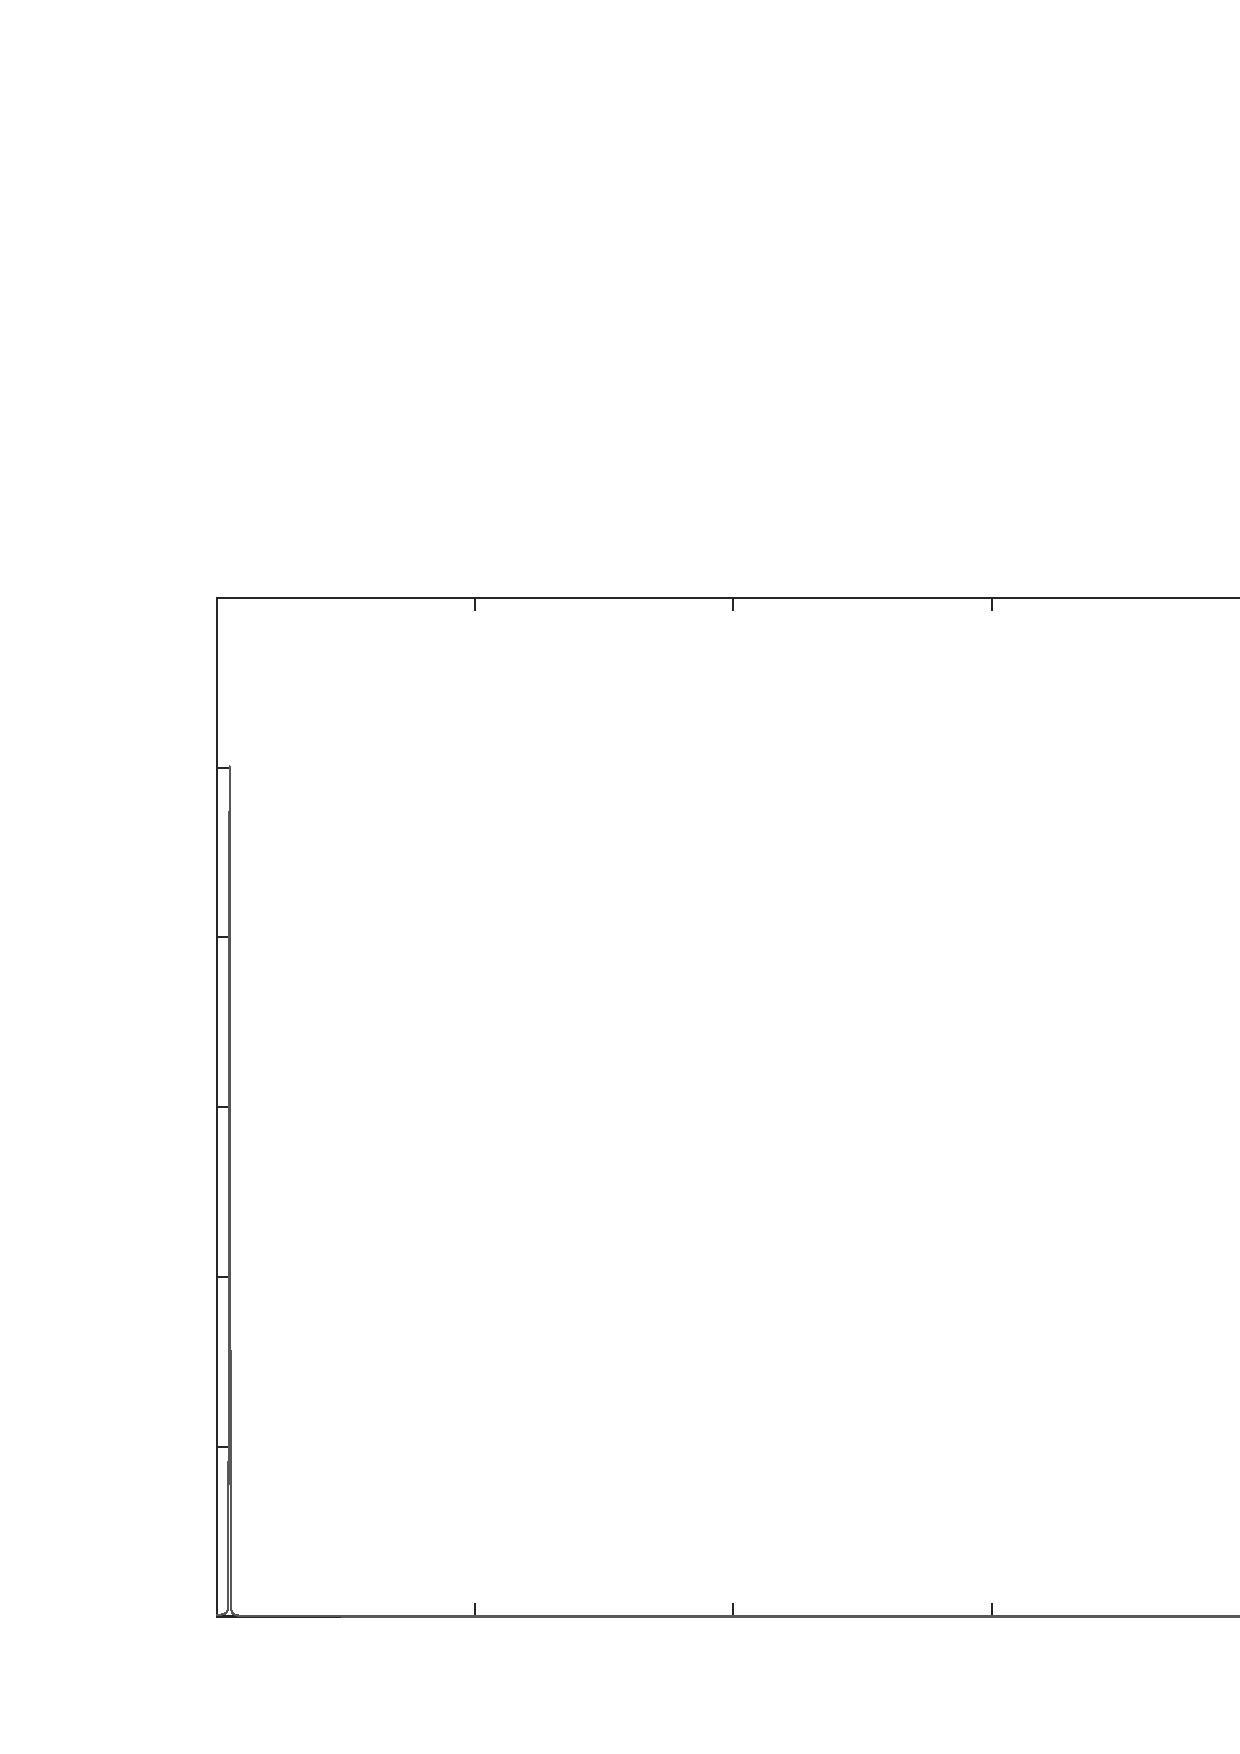
\includegraphics[scale=1]{octaves/cosineFT-inc}
\end{picture}%
\begin{picture}(800,600)(0,0)
\fontsize{13}{0}\selectfont\put(104,55.5788){\makebox(0,0)[t]{\textcolor[rgb]{0.15,0.15,0.15}{{0}}}}
\fontsize{13}{0}\selectfont\put(228,55.5788){\makebox(0,0)[t]{\textcolor[rgb]{0.15,0.15,0.15}{{0.2}}}}
\fontsize{13}{0}\selectfont\put(352,55.5788){\makebox(0,0)[t]{\textcolor[rgb]{0.15,0.15,0.15}{{0.4}}}}
\fontsize{13}{0}\selectfont\put(476,55.5788){\makebox(0,0)[t]{\textcolor[rgb]{0.15,0.15,0.15}{{0.6}}}}
\fontsize{13}{0}\selectfont\put(600,55.5788){\makebox(0,0)[t]{\textcolor[rgb]{0.15,0.15,0.15}{{0.8}}}}
\fontsize{13}{0}\selectfont\put(724,55.5788){\makebox(0,0)[t]{\textcolor[rgb]{0.15,0.15,0.15}{{1}}}}
\fontsize{13}{0}\selectfont\put(97.0525,66){\makebox(0,0)[r]{\textcolor[rgb]{0.15,0.15,0.15}{{0}}}}
\fontsize{13}{0}\selectfont\put(97.0525,147.5){\makebox(0,0)[r]{\textcolor[rgb]{0.15,0.15,0.15}{{100}}}}
\fontsize{13}{0}\selectfont\put(97.0525,229){\makebox(0,0)[r]{\textcolor[rgb]{0.15,0.15,0.15}{{200}}}}
\fontsize{13}{0}\selectfont\put(97.0525,310.5){\makebox(0,0)[r]{\textcolor[rgb]{0.15,0.15,0.15}{{300}}}}
\fontsize{13}{0}\selectfont\put(97.0525,392){\makebox(0,0)[r]{\textcolor[rgb]{0.15,0.15,0.15}{{400}}}}
\fontsize{13}{0}\selectfont\put(97.0525,473.5){\makebox(0,0)[r]{\textcolor[rgb]{0.15,0.15,0.15}{{500}}}}
\fontsize{13}{0}\selectfont\put(97.0525,555){\makebox(0,0)[r]{\textcolor[rgb]{0.15,0.15,0.15}{{600}}}}
\end{picture}

    }\caption{Plot of the Fourier Transform of \texttt{cos(2*pi*x)}. The two
    impulses are located very close to $0$ and $1$.}\label{oct:cosineFT}
\end{center}
\end{figure*}

\begin{figure*}[ht]
\begin{center}
\scalebox{0.5}{
% Title: gl2ps_renderer figure
% Creator: GL2PS 1.4.2, (C) 1999-2020 C. Geuzaine
% For: Octave
% CreationDate: Mon Oct 31 14:18:23 2022
\setlength{\unitlength}{1pt}
\begin{picture}(0,0)
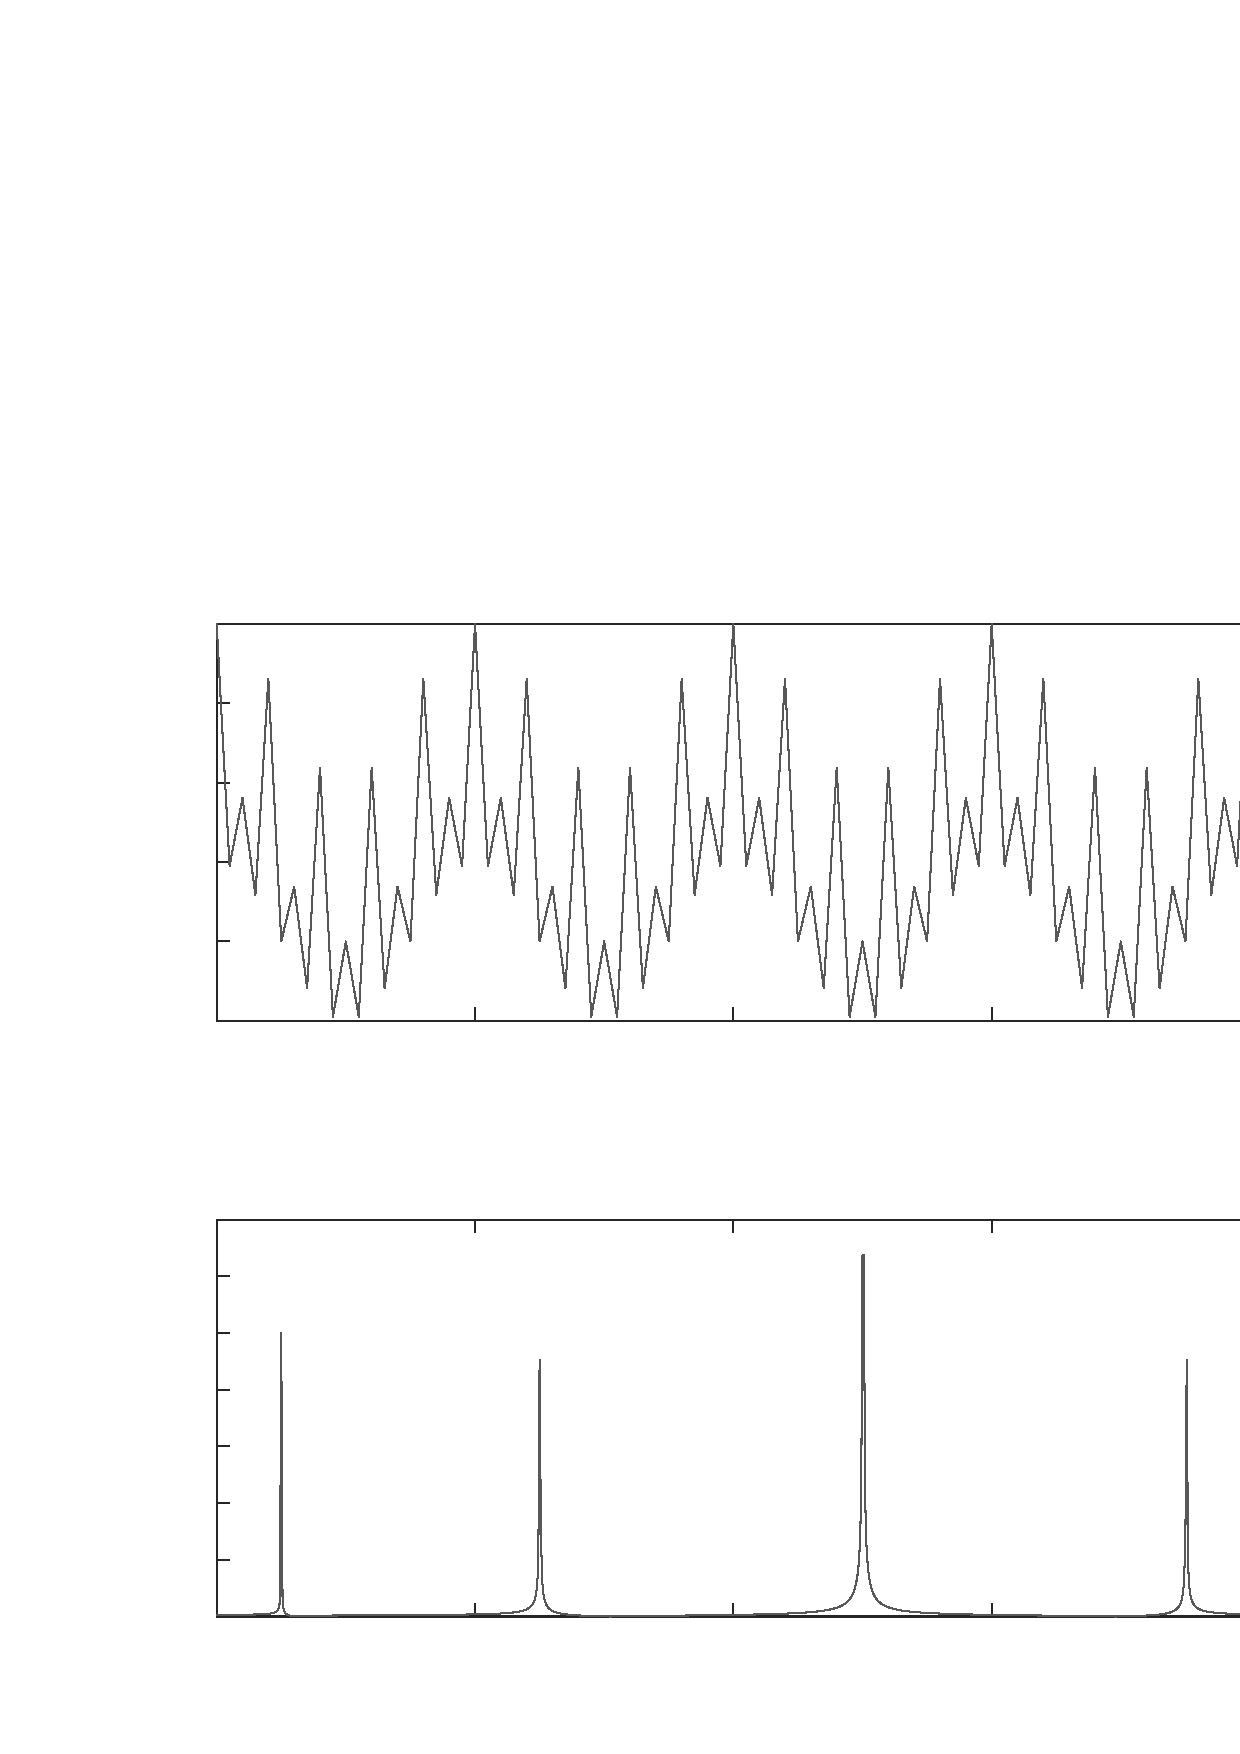
\includegraphics[scale=1]{octaves/cosineSumFT-inc}
\end{picture}%
\begin{picture}(800,600)(0,0)
\fontsize{13}{0}\selectfont\put(104,341.475){\makebox(0,0)[t]{\textcolor[rgb]{0.15,0.15,0.15}{{0}}}}
\fontsize{13}{0}\selectfont\put(228,341.475){\makebox(0,0)[t]{\textcolor[rgb]{0.15,0.15,0.15}{{0.2}}}}
\fontsize{13}{0}\selectfont\put(352,341.475){\makebox(0,0)[t]{\textcolor[rgb]{0.15,0.15,0.15}{{0.4}}}}
\fontsize{13}{0}\selectfont\put(476,341.475){\makebox(0,0)[t]{\textcolor[rgb]{0.15,0.15,0.15}{{0.6}}}}
\fontsize{13}{0}\selectfont\put(600,341.475){\makebox(0,0)[t]{\textcolor[rgb]{0.15,0.15,0.15}{{0.8}}}}
\fontsize{13}{0}\selectfont\put(724,341.475){\makebox(0,0)[t]{\textcolor[rgb]{0.15,0.15,0.15}{{1}}}}
\fontsize{13}{0}\selectfont\put(97.0525,351.924){\makebox(0,0)[r]{\textcolor[rgb]{0.15,0.15,0.15}{{-2}}}}
\fontsize{13}{0}\selectfont\put(97.0525,390.024){\makebox(0,0)[r]{\textcolor[rgb]{0.15,0.15,0.15}{{-1}}}}
\fontsize{13}{0}\selectfont\put(97.0525,428.124){\makebox(0,0)[r]{\textcolor[rgb]{0.15,0.15,0.15}{{0}}}}
\fontsize{13}{0}\selectfont\put(97.0525,466.224){\makebox(0,0)[r]{\textcolor[rgb]{0.15,0.15,0.15}{{1}}}}
\fontsize{13}{0}\selectfont\put(97.0525,504.324){\makebox(0,0)[r]{\textcolor[rgb]{0.15,0.15,0.15}{{2}}}}
\fontsize{13}{0}\selectfont\put(97.0525,542.424){\makebox(0,0)[r]{\textcolor[rgb]{0.15,0.15,0.15}{{3}}}}
\fontsize{15}{0}\selectfont\put(414,552.424){\makebox(0,0)[b]{\textcolor[rgb]{0,0,0}{{Sum of cosines}}}}
\fontsize{13}{0}\selectfont\put(104,55.5514){\makebox(0,0)[t]{\textcolor[rgb]{0.15,0.15,0.15}{{0}}}}
\fontsize{13}{0}\selectfont\put(228,55.5514){\makebox(0,0)[t]{\textcolor[rgb]{0.15,0.15,0.15}{{0.2}}}}
\fontsize{13}{0}\selectfont\put(352,55.5514){\makebox(0,0)[t]{\textcolor[rgb]{0.15,0.15,0.15}{{0.4}}}}
\fontsize{13}{0}\selectfont\put(476,55.5514){\makebox(0,0)[t]{\textcolor[rgb]{0.15,0.15,0.15}{{0.6}}}}
\fontsize{13}{0}\selectfont\put(600,55.5514){\makebox(0,0)[t]{\textcolor[rgb]{0.15,0.15,0.15}{{0.8}}}}
\fontsize{13}{0}\selectfont\put(724,55.5514){\makebox(0,0)[t]{\textcolor[rgb]{0.15,0.15,0.15}{{1}}}}
\fontsize{13}{0}\selectfont\put(97.0525,66){\makebox(0,0)[r]{\textcolor[rgb]{0.15,0.15,0.15}{{0}}}}
\fontsize{13}{0}\selectfont\put(97.0525,93.2143){\makebox(0,0)[r]{\textcolor[rgb]{0.15,0.15,0.15}{{100}}}}
\fontsize{13}{0}\selectfont\put(97.0525,120.429){\makebox(0,0)[r]{\textcolor[rgb]{0.15,0.15,0.15}{{200}}}}
\fontsize{13}{0}\selectfont\put(97.0525,147.643){\makebox(0,0)[r]{\textcolor[rgb]{0.15,0.15,0.15}{{300}}}}
\fontsize{13}{0}\selectfont\put(97.0525,174.857){\makebox(0,0)[r]{\textcolor[rgb]{0.15,0.15,0.15}{{400}}}}
\fontsize{13}{0}\selectfont\put(97.0525,202.071){\makebox(0,0)[r]{\textcolor[rgb]{0.15,0.15,0.15}{{500}}}}
\fontsize{13}{0}\selectfont\put(97.0525,229.286){\makebox(0,0)[r]{\textcolor[rgb]{0.15,0.15,0.15}{{600}}}}
\fontsize{13}{0}\selectfont\put(97.0525,256.5){\makebox(0,0)[r]{\textcolor[rgb]{0.15,0.15,0.15}{{700}}}}
\fontsize{15}{0}\selectfont\put(414,266.5){\makebox(0,0)[b]{\textcolor[rgb]{0,0,0}{{Fourier Transform}}}}
\end{picture}

    }\caption{Signal $c(x) = \cos{2\pi 5 x} + \cos{2\pi 25 x} + \cos{2\pi 50x}$
    and its Fourier Transform. The resulting Fourier Transform, obtained with
    function \texttt{fft()}, is the superposition of three distinct
    frequencies, each related to one of the three sinusoids forming signal
    $c(x)$.}\label{oct:cosineSumFT}
\end{center}
\end{figure*}

Classic Fourier Transforms suffer from crucial limitations. Undeniably, due to the uncertainty principle they cannot provide \emph{simultaneous} time and frequency localization. This means that, for instance, delta impulses in the frequency domain are likely generated by very long, if not infinite, sinusoids in the time domain---vice versa, brief signals in the time domain will yield a Fourier Transform with a very large band. In addition, they are not exactly useful for analyzing \emph{time-variant, non-stationary} signals\footnote{ Time-variant, non-stationary signals are the class of signals whose spectrum changes overtime.}, as the frequency of such signals or sequences is subject to possible variations whilst the content of the signal alters across time, resulting in a confusing frequency description.

Typically, noise in Fourier Transform is caused by abrupt changes in frequency of the signal---the more sudden the change in the speed of oscillation of the signal, the greater the noise will be produced. The result frequency description is still an faithful portrait of the signal's frequency content; still, added noise and multiple frequencies due to the non-stationary nature of the considered signal will yield a chaotic Fourier Transform which is hard to interpret.

The answer to this issue is the \textbf{Short Time Fourier Transform}, abbreviated in STFT. The key concept behind the short time Fourier Transform is to appropriately segment the time-variant signal into narrow time intervals, thin enough that the portion of the signal in it can be considered stationary. For each segment, perform a Fourier Transform of it: each Fourier Transform will provide the spectral information of a separate segment of the signal, yielding \emph{simultaneous} time and frequency information.

This means that the STFT involves computing the frequency description of the
time-domain segment \emph{and} keeping the information on which segment has
been transformed. In other words, the steps can be summarized as:
\begin{enumerate}
    \item choose a window function $W(t)$ of finite length, in order to select a
        narrow portion of the original signal;
    \item start with the window at position $t = 0$;
    \item truncate the signal with the window to obtain a segment of the
        original signal;
    \item compute the Fourier Transform of the segment, conveniently store the
        result;
    \item incrementally slide the window of $t'$ to the right, as needed, hence
        obtain $W(t - t')$;
    \item go to step $3$ until the window has covered the entire signal;
\end{enumerate}

Operating such procedure will yield results that can be collected in a data
structure; each Fourier Transform can be mathematically described in the following manner,
\begin{equation}\label{eqn:shortTimeFourierTransform}
    \mathrm{STFT}^u_f(t', u) = \int_t \left[f(t) \cdot W(t - t')\right]e^{-j2\pi ut}dt,
\end{equation}
where $t'$ is the \emph{time parameter} that controls the amount of shifting the window is subject to, $u$ is the frequency parameter, $f$ is the original signal $f(t)$, $W(t)$ is the windowing function, centered at $t = t'$. In brief, the operation involved is the transform of the signal $f(t)W(t - t')$ with the frequency variable $u$.

The windowing function is free to choose as desired. The shape of it could be rectangular, Gaussian, triangular, and so on. The window should be narrow enough to ensure that the portion of the signal falling withing the window \emph{is stationary}, but at the same time very narrow windows offer \emph{poor localization} in the frequency domain. This is because the Short Time Fourier Transform, as with any other Fourier Transform, is heavily dependent on the uncertainty principle---as such, there is a trade--off between \emph{localization in the frequency domain} and \emph{localization in the time domain}.

A choice of $W(t)\equiv 1$ would yield an infinitely long window: the STFT turns into a simple FT, providing exemplary frequency localization but nonexistent time localization. On contrary, a choice of $W(t) = \delta(t)$ would yield an infinitesimally short window, resulting in the time signal itself\footnote{In fact, 
\[
    \mathrm{STFT}^u_f(t', u) = \int_t \left[f(t) \cdot \delta(t - t')\right]e^{-j2\pi ut}dt = f(t')e^{-jut'},
\] with a single $f(t')$ transformed.}---but with a phase factor added---providing maximal time localization, but vacant frequency localization. Anything in between will yield a compromise between the two extremes, with wide windows assuring good frequency and poor time resolution, and narrow windows providing good time resolution at the expense of the frequency resolution.

It is clear that, especially in the case of signals whose content changes \emph{a lot} during time, a single window choice cannot possibly fit the entire signal and describe it efficiently. A way to overcome this limitation is to use the \textbf{wavelets}. Wavelets technique makes use of \emph{multiple window sizes} in order to catch various facets of the signal to analyze, capable of adjusting to the time-varying frequency. In order to localize frequency, a decent amount of signal should be processed---but the larger the span, the fewer the time localization.

The \textbf{uncertainty principle} was mathematically coded by scientist \emph{Werner Heisenberg} in 1927, and is any of a variety of mathematical inequalities asserting a fundamental limit to the accuracy with which the values for certain pairs of physical quantities of a particle, such as position, $x$, and momentum, $p$, can be predicted from initial conditions\cite{bib:wernerHeisemberg}.

Such variable pairs are known as complementary variables or canonically conjugate variables; and, depending on interpretation, the uncertainty principle limits to what extent such conjugate properties maintain their approximate meaning, as the mathematical framework of quantum physics does not support the notion of simultaneously well-defined conjugate properties expressed by a single value. The uncertainty principle implies that it is in general not possible to predict the value of a quantity with arbitrary certainty, even if all initial conditions are specified\cite{bib:wernerHeisemberg}.

Related to digital signal processing, the uncertainty principle gathers in the
form of
\begin{equation}\label{eqn:uncertaintyPrinciple}
    \Delta t \cdot \Delta f \geq \frac 1 {4\pi},
\end{equation}
where $\Delta t$ is the \emph{time resolution}---how well two spikes in time can be separated from each other in the frequency domain---and $\Delta f$ is the \emph{frequency resolution}---how well two spectral components can be divided from each other in the time domain. The unquestionable fact is that \emph{both $\Delta t$ and $\Delta f$ cannot be made arbitrarily small}: shrinking one of the two will incontrovertibly grow the other, and vice versa!

This fundamental law of nature can never be infringed, signifying that one cannot know the \emph{exact} time-frequency representation of a signal, since it must abide to the uncertainty principle and will be subject to a trade--of between time resolution and frequency resolution: one can only know what inverval of frequencies belongs to a given time interval. Wavelets are windows whose value take in account the product $\Delta t \Delta f$, and can be represented by rectangles having base $\Delta f$ and height $\Delta t$. The area of the wavelets cannot go below the value $\Delta t \cdot \Delta f$.
